\documentclass[grado3]{LEMA-Tikz-IM}

\usepackage{graphicx}  % Needed to include graphics
\usepackage{pifont} % For the scissors symbol

\begin{document}
\begin{tikzpicture}
% \pgfplotsset{compat=1.18}

% page canvas letter size
\path (0,0) rectangle (8.5in,11in);

% draw cut line
\usetikzlibrary{decorations.text}
\node at (0.5in, 11in/2) {\scalebox{2}{\ding{36}}};
\node at (8.5in-0.5in, 11in/2) {\scalebox{2}{\ding{36}}};
\draw[dashed, line width=1pt] (0,11in/2) -- (8.5in, 11in/2);

\def\myMargin{1in}

\coordinate (botLeft) at (\myMargin,\myMargin);
\coordinate (botRight) at (8.5in-\myMargin,\myMargin);
\coordinate (topRight) at (8.5in-\myMargin,11in-\myMargin);
\coordinate (topLeft) at (\myMargin,11in-\myMargin);

% clip outside the margin 
\draw (botLeft) rectangle (topRight);

% draw middle line
\coordinate (midLeft) at ($ (botLeft)!0.5!(topLeft) $);
\coordinate (midRight) at ($ (botRight)!0.5!(topRight) $);
\draw (midLeft)  -- (midRight);

% find center of top and bottom parts of the page
\coordinate (centerTop) at ($ (midLeft)!0.5!(topRight) $);
\coordinate (centerBot) at ($ (midLeft)!0.5!(botRight) $);

% add tables to top and bottom
\node (tableTop) at ([yshift=-3ex]centerTop) {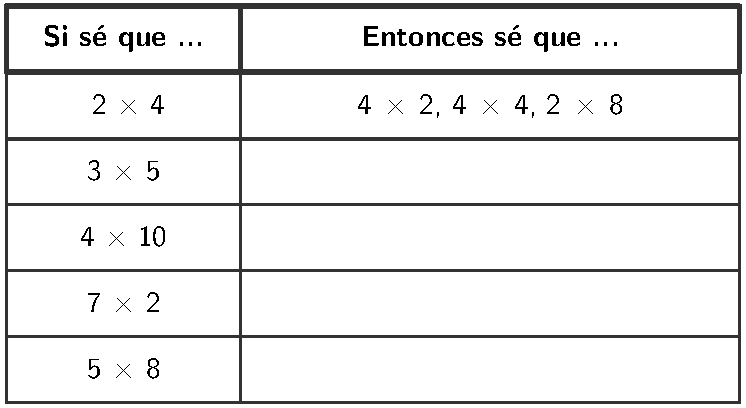
\includegraphics{siSeQueEntoncesSeQueMult-BLM-tab-para2copias.pdf}};
\node (tableBot) at ([yshift=-3ex]centerBot) {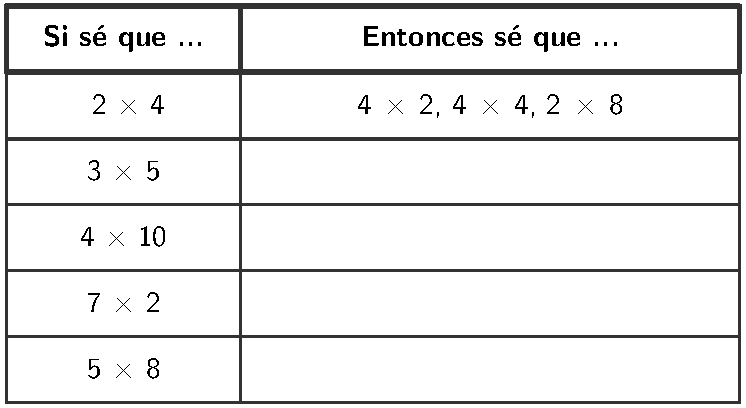
\includegraphics{siSeQueEntoncesSeQueMult-BLM-tab-para2copias.pdf}};

% Add png decoration to top and bottom
% \node[above] at (tableTop.north) {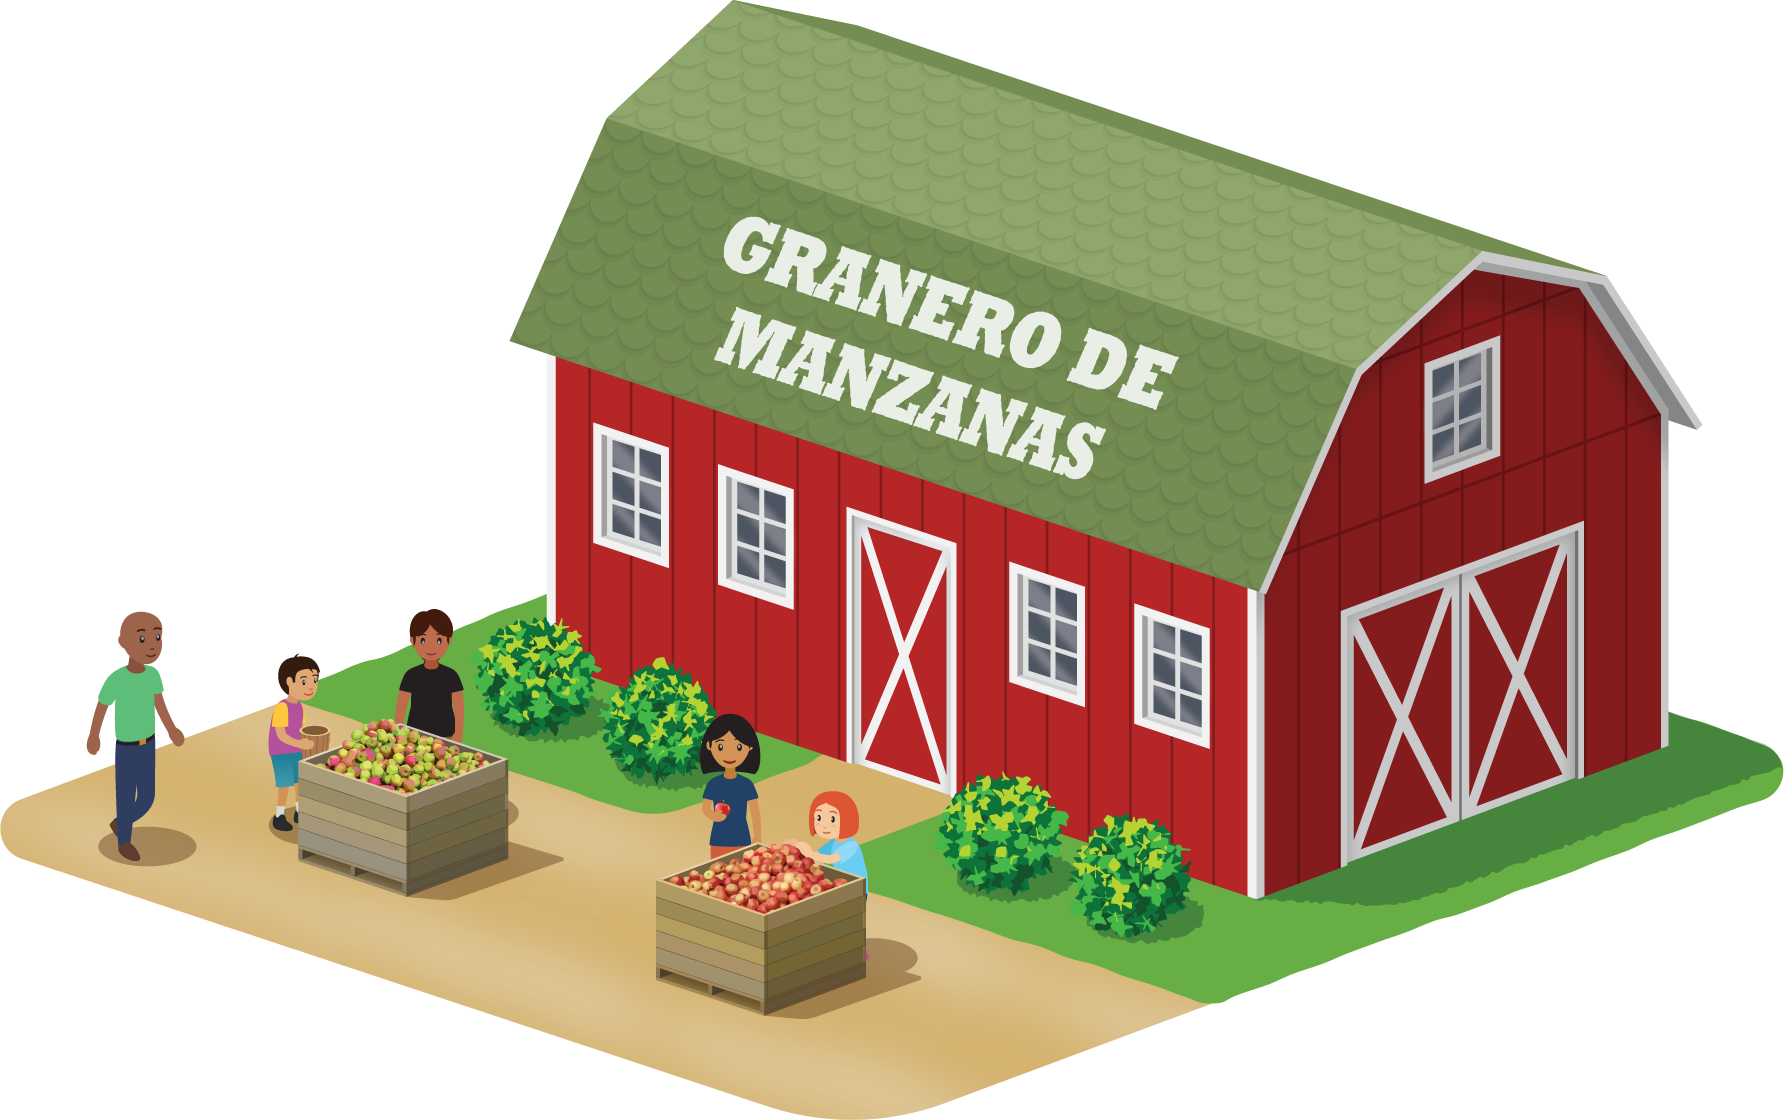
\includegraphics[width=3.5cm]{../../png-source/3.4.D21.S_Sp.png}};
% \node[above] at (tableBot.north) {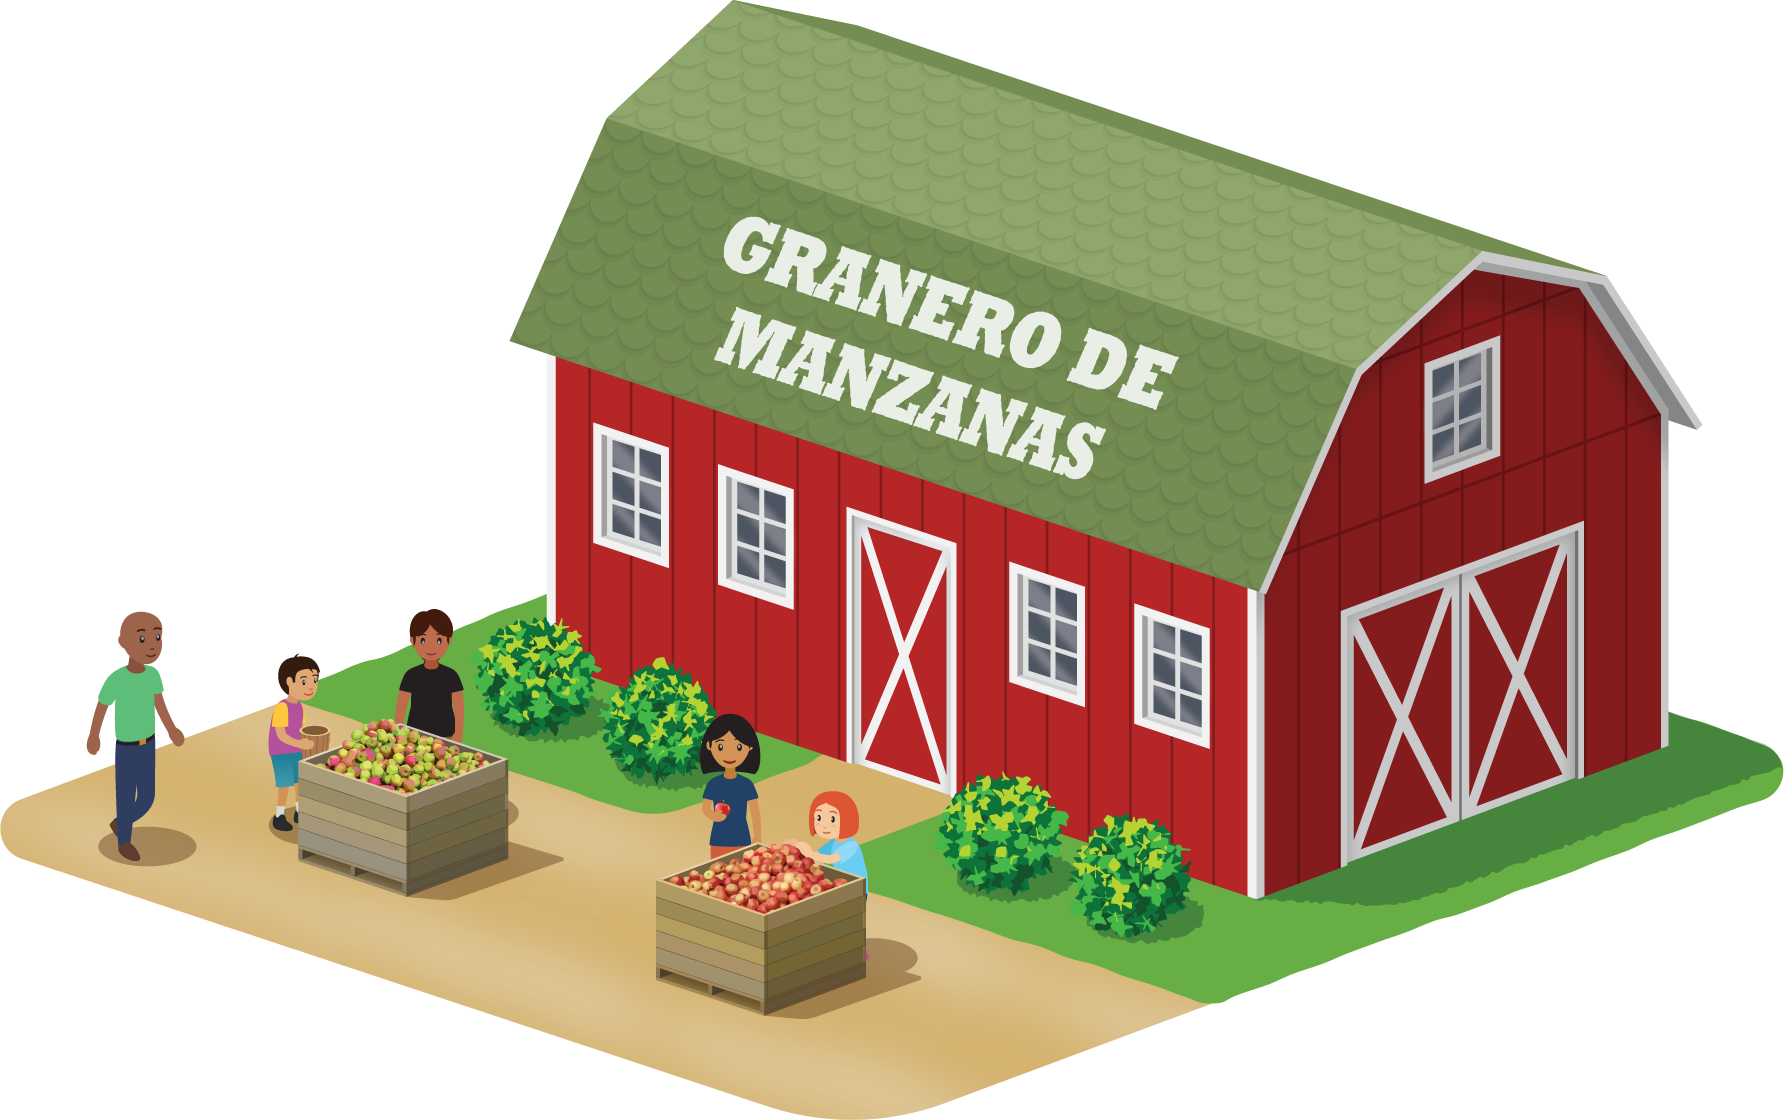
\includegraphics[width=3.5cm]{../../png-source/3.4.D21.S_Sp.png}};

% Add BLM heading to top and bottom
\node[below right, align=left, font=\bf] at (topLeft) {Si sé que ..., entonces sé que ...\\Multiplicación};
\node[below right, align=left, font=\bf] at (midLeft) {Si sé que ..., entonces sé que ...\\Multiplicación};


% Espacio de nombre
\node[below left] at ([yshift=-5ex]topRight) {Nombre: \underline{\hspace{6cm}}};
\node[below left] at ([yshift=-5ex]midRight) {Nombre: \underline{\hspace{6cm}}};



\end{tikzpicture}
\end{document}